As the lines were synthetic, we had access to both a mask (\fref{f:synth_mammography}b) and ground truth orientation for the superimposed structure.

Unlike other similar studies~\cite{Berks_etal_IPMI11}, we do not require a negative classification of background pixels and therefore do not need to remove existing real structures from the images. As a result, the synthetic lines will be disrupted by any existing image structure and thus the dataset presents a much tougher and more realistic test of orientation estimation than shown in, for example,~\cite{Berks_etal_IPMI11}.

We sampled 200\,000 pixels from such images and computed a feature vector for each with which we trained a regressor. We then applied every trained regressor for every feature type to a fixed set of 100 synthesized images (generated from mammographic backgrounds not used in training) and computed the error at the known line pixel positions. As before, Random Forests and the \dtcwt{} outperform other methods, though errors were generally higher on account of the more challenging data (\fref{f:mammo_graphs}a and \tref{t:synth_mammography}). We also note that although the median error for the Random Forest was lower for the \dtcwt~than the second derivatives, the situation was reversed for higher percentiles (\ie~the graphs cross). We care less, however, about differences between errors above a certain threshold (it matters little whether the estimate is out by $60^\circ$ or $70^\circ$ -- they are both terrible estimates) so it may be argued that the Random Forest performs better over the region in which we are interested.

For orientation, only pixels belonging to curvilinear structures (although not necessarily at the centerline) were included in the results. The absolute differences between the predicted and known orientations (with appropriate angle wrapping) were taken, and used to generate cumulative distribution functions of orientation errors for each method, as shown in~\ref{f:}. The mean absolute errors of the estimated orientations are also included in~\ref{t:}.

%\input{figs/fig_synth_mammograms.tex}
%% CVPR Figure 5

\begin{figure}[t]
\centering
\begin{tabular}{@{}c c@{}}
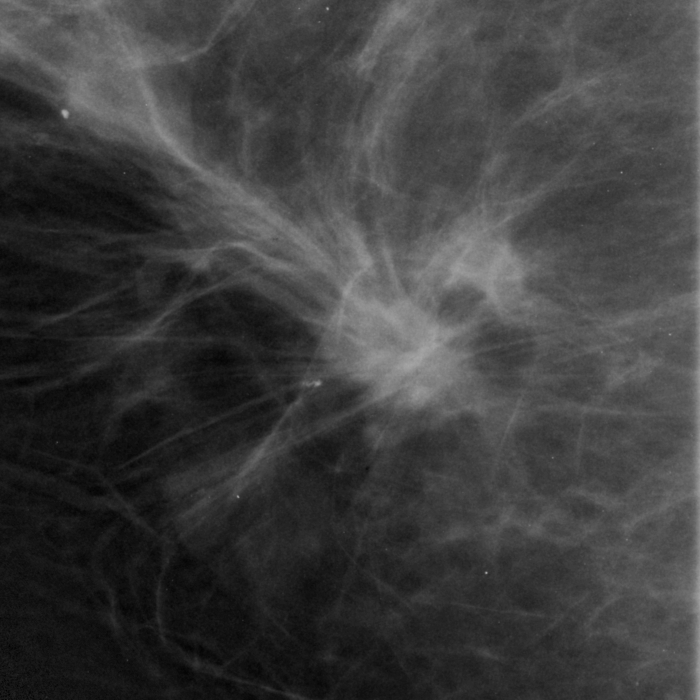
\includegraphics[width=0.47\columnwidth]{\figpath/mammo/024RCC_roi_crop} &
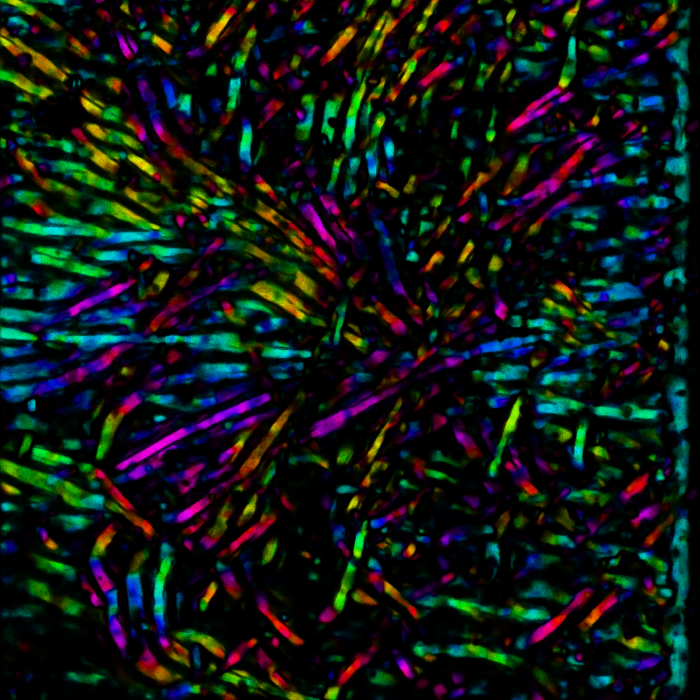
\includegraphics[width=0.47\columnwidth]{\figpath/mammo/024RCC_roi_class_ori_crop} \\
(a) & (b) \\
\noalign{\smallskip}
\end{tabular}
%
\caption{Real mammographic images: %
(a) input image; %
(b) estimated orientation from a Random Forest using \dtcwt{} features. Hue indicates the estimated orientation and brightness is determined by the confidence in the estimate (as quantified by the magnitude of the predicted orientation vector).}
\label{f:real_mammography}
\end{figure}

%\begin{table}[t]
\centering
\begin{tabular}{l c c c c}
\toprule
							& \multicolumn{4}{c}{Feature Type} \\
							& $G'$		& $G''$	& Mono.				& \dtcwt \\
\cmidrule{2-5}
\input{mammography_table.txt}
\bottomrule
\noalign{\smallskip}
\end{tabular}
%
\caption{Median absolute error (degrees) for combinations of input feature and {3{$\times$}3} regressor on 100 synthetic mammogram images.}
\label{t:synth_mammography}
\end{table}

%CVPR Figure 4

\begin{figure}[t]
\centering
\begin{tabular}{c c}
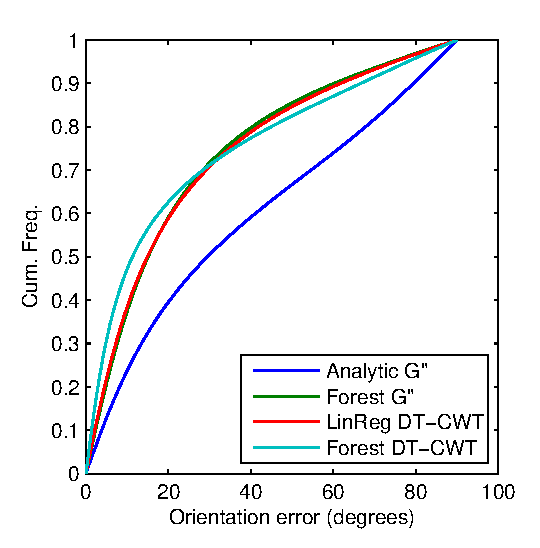
\includegraphics[width=0.47\columnwidth]{\figpath/mammo/cdf_error_mammo} &
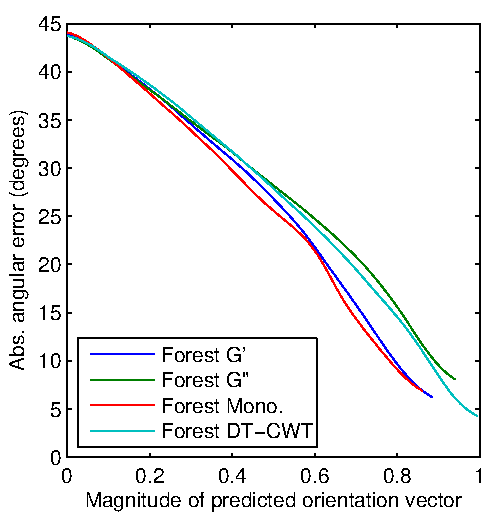
\includegraphics[width=0.46\columnwidth]{\figpath/mammo/response_vs_error_mammo} \\
(a) & (b) \\
\noalign{\smallskip}
\end{tabular}
%
\caption{Mammogram results for four selected methods: (a) Cumulative frequency of angular error; (b) Kernel estimate of mean error with respect to the magnitude of the orientation vector predicted by the forest.}
\label{f:mammo_graphs}
\end{figure}


In \fref{f:mammo_graphs}b we show the kernel estimate of mean angular error with respect to the magnitude of the orientation vector predicted by the forest trained on each feature type. Recall that this magnitude encodes the mean angular dispersion of the training data arriving the leaf nodes used in making each orientation prediction. That this magnitude acts as a measure of confidence in its prediction is evidenced by consistent reduction in angular error with increasing magnitude for all feature types. The magnitudes can be used to weight each orientation prediction in further processing and may be preferable to a similar feature such as the absolute response returned from the analytic combination of the Gaussian derivatives. This is because the latter is essentially a measure of image contrast at a structure of interest. So for example, if there are two lines, one of which has double the contrast of the other, the magnitude of the filter response will also double, even if the orientation may measured equally accurately in both lines. Similarly, a very bright or very dark spot in the image will also produce a strong filter response where in fact orientation can't be reliably estimated.

% CLAIM: that the separable filters are faster than nonseparable ones (but by how much?)
% CLAIM: that the Haar-like features are faster than separable filtering
In terms of efficiency, we recorded the mean time (using Matlab on a 2.66Ghz, quad-core desktop PC with 3.25Gb RAM) over 20 images for five feature representations: 
the monogenic signal (2.96\emph{s}); 
%non-separable second derivatives (3.71\emph{s}); 
separable second derivatives (2.04\emph{s}); 
%their Haar-like approximations (2.35\emph{s}); 
and the \dtcwt{} (19.96\emph{s}). 
%
Unsurprisingly, under test conditions 
%the separable filters were indeed faster than their non-separable counterparts while 
the \dtcwt{} was an order of magnitude slower than the separable filters. 
%
%The Haar-like approximations were comparable to but slower than the separable filters, though the separable filters did exploit the built-in (\ie~compiled) convolution functions in Matlab; we expect that an optimized implementation of the Haar-like features would offer similar performance gains as observed in face detection applications~\cite{Viola_Jones_IJCV04}.
%
%%% This is a pretty weak conclusion to the experiment but the best we can expect at this point. Also, if you need to use a regressor as slow as the RF to get accuracy that is comparable to the analytic second derivatives then the small difference in filtering time becomes irrelevant}

%begin IPMI
The orientation results for both Monogenic and Monogenic/RF were surprisingly poor. Counter-intuitively, visual analysis of the test outputs showed that the Monogenic methods performed particularly badly at the exact centerline of curvilinear structures, where an essentially random orientation appeared to be returned. This is in contrast to the other tested methods that, as expected, performed strongest along the centerlines of structures. Computing estimation errors at pixels belonging to structures but not lying on the centerline produces a small improvement in the results (mean absolute errors of $32.55 \deg$ and $29.39 \deg$ for the RF and prescriptive variant respectively), though even then performance lags behind the other tested methods and of course in a real image we do not know the precise location of structure centerlines. 
%end IPMI